\documentclass[12pt]{article}

\usepackage[english]{babel}
\usepackage[utf8]{inputenc}
\usepackage[T1]{fontenc}
\usepackage{graphicx}
\usepackage{amsmath}
\usepackage{fancyhdr}
\usepackage{siunitx}
\usepackage{listings}

\makeatletter
\def\@seccntformat#1{\csname the#1\endcsname\hspace*{0.5em}$|$\hspace*{0.5em}}
\makeatother

\pagestyle{fancy}

\title{\textbf{Quartz resonator} \\ SCI-C0200}
\author{Joonatan Bergholm 507260 \\ Osama Abuzaid XXXXXX}

\begin{document}

\pagenumbering{gobble}
\maketitle
\newpage

\pagenumbering{arabic}

\tableofcontents
\newpage

\section{Introduction}

In this assignment we investigated electronic properties of one of the most common electronic components, the quartz tuning fork or quartz resonator, like one in figure \ref{fig:kvres}. It is used in watches and other every day electrical appliances to provide a stable clocking frequency. Typically the frequency is $f_0 = \SI{32768}{\hertz}$, because is is a round number ($32768_{10} = {2^{15}}_{10} = 1000000000000000_2$) in base 2, which is commonly used in electrical appliances.

Contrary to conventional tuning fork, one does not need generate mechanical excitation
on the quartz tuning fork, because quartz has piezoelectric properties and thus mechanical excitation can be replaced with electronic one.

\section{Theory}

\begin{figure}
	\centering
	\includegraphics[width = \textwidth]{kuvat/kvres.png}
	\caption{Quartz resonator}
	\label{fig:kvres}
\end{figure}

\section{Results}

\begin{figure}
	\centering
	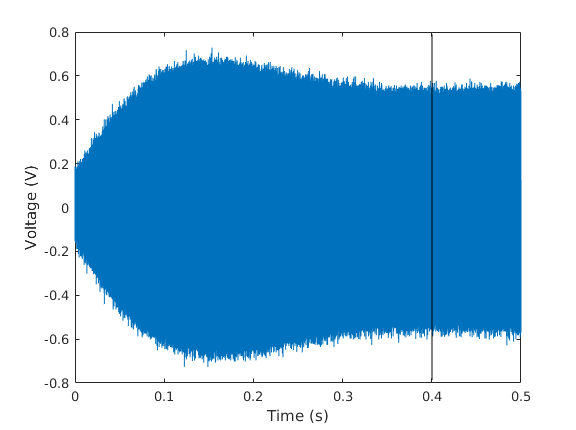
\includegraphics[width = \textwidth]{kuvat/steadystate.png}
	\caption{Steady state}
	\label{fig:steady}
\end{figure}

\appendix

\section{Source code}

\lstinputlisting[caption = ac.m]{matlab/ac.m}
%\lstinputlisting[caption = ac.m]{matlab/DAQreadout.m}

\end{document}